% Chapter Template

\chapter{Ensayos y resultados} % Main chapter title

\label{Chapter4} % Change X to a consecutive number; for referencing this chapter elsewhere, use \ref{ChapterX}

%----------------------------------------------------------------------------------------
%	CHAPTER 4
%----------------------------------------------------------------------------------------

En este capítulo se explica cómo se llevaron a cabo las pruebas de validación de hardware y software a las que fue sometido el dispositivo, los bancos de ensayos, instrumentos utilizados y los resultados obtenidos.

\section{Instrumental utilizado}

Para poder ejecutar las pruebas de integración de hardware y software se requirió del uso de una variedad de instrumentos y componentes en los bancos de ensayos. La tabla \ref{tab:instrumentos} lista los detalles de cada uno de ellos.

\begin{table}[H]
	\centering
	\caption{Lista de instrumental utilizado.}
	\begin{tabular}{p{3cm} c p{6cm}}
		\toprule
		\textbf{Item} & \textbf{Modelo} & \textbf{Descripción} \\
		\midrule
		Multímetro			& UNI-T UT61A		& Multímetro digital autorango de alta precisión. \\
		Fuente de tensión	& KM GP-300ATX		& Fuente de computadora de 400 W. \\
		Resistencia de potencia variable		& AVT05006E25R00KE	& Resistencia de potencia de alambre bobinado de 25 Ohm / 50 W. \\
		Potenciómetro							& 3590S-1-201L & Potenciómetro de 200 Ohm / 2 W y 10 vueltas para panel. \\
		Conversor USB a UART					& EM7-6043		& Conversor USB a serie TTL CH-340. \\
		Cables varios							& - 			& Cables dupont y unipolar de 2,5 mm\textsuperscript{2}. \\
		PC										& -				& Computadora de escritorio con software PuTTY (cliente de terminal). \\
		\bottomrule
		\hline
	\end{tabular}
	\label{tab:instrumentos}
\end{table}

En el apéndice \ref{AppendixB} se puede ver una foto del banco de ensayos completo con todos los instrumentos y hardware utilizado.

\section{Pruebas de hardware}
\label{sec:pruebasHW}

Para validar el funcionamiento del hardware, basta con medir continuidad o niveles de tensión en ciertos puntos de la placa. Por esta razón, se omite especificar las pruebas a excepción de las del monitor de corriente, ya que es el único caso en el que es necesario realizar mediciones.

\subsection{Prueba del monitor de corriente}
\label{sec:monCorr}

En el circuito del monitor de corriente lo que se desea verificar es que a la salida del amplificador se obtenga una tensión proporcional al valor de corriente que circula. La constante de conversión surge de multiplicar el valor de la resistencia de sensado (10 mOhm) por la constante de amplificación del circuito integrado (100 V/V), lo que resulta en un valor de 1 V/A. Por lo tanto, la conversión entre corriente y tensión es unitaria.

Para realizar las mediciones se conecta la entrada de tensión a la fuente de 5 V, una resistencia de potencia en la salida de tensión y se varía su valor de forma de hacer circular desde 0 A hasta aproximadamente 3,3 A.

%\begin{figure}[H]
%\centering
%\includegraphics[width=0.9\textwidth]{./Figures/esqMonCorr.png}
%\caption{Esquema de medición del monitor de corriente.}
%\label{fig:esqMonCorr}
%\end{figure}

Con los datos obtenidos se calcula para cada medición el error porcentual con respecto al valor teórico de la constante de conversión. En la figura \ref{fig:testMonCorr} se pueden ver los valores computados para distintos valores de corriente en la carga.

\begin{figure}[H]
\centering
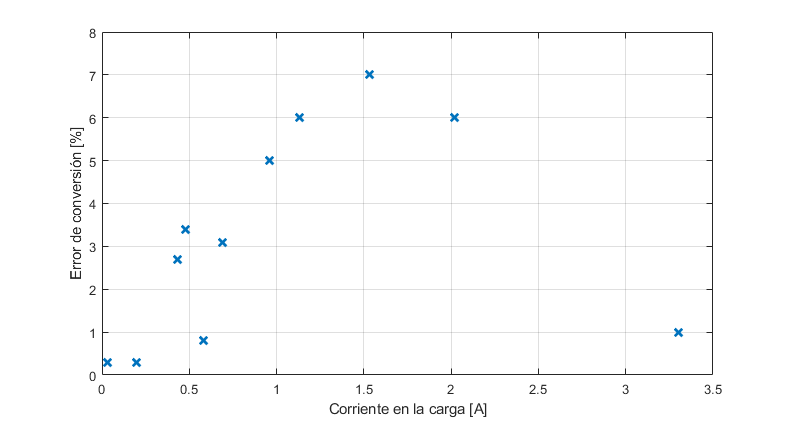
\includegraphics[width=0.9\textwidth]{./Figures/testMonCorr.png}
\caption{Error porcentual de la constante de conversión de corriente.}
\label{fig:testMonCorr}
\end{figure}

Del gráfico se observa que en este rango se tiene un error de medición máximo del 7 \% y un valor promedio aproximado del 3,23 \% respecto del valor real.

Esta diferencia entre el valor de la constante medida y el teórico se la puede atribuir principalmente a dos efectos: la dispersión del valor de la resistencia de sensado y a la presencia de ruido en el circuito. El error de la ganancia del circuito integrado está especificado en un máximo de 0,2\% por lo que no aporta variaciones significativas.

\section{Pruebas de firmware}
\label{sec:pruebasFW}

Las pruebas de firmware tienen como finalidad validar el funcionamiento individual de una biblioteca o una parte en particular del código desarrollado. Para ello, en algunos casos lo que se hace es directamente mostrar funcionalidades específicas del programa funcionando, como por ejemplo en el driver de la pantalla LCD y de la consola de control.

\subsection{Prueba del monitor de tensión}

Para el monitor de tensión y el monitor de corriente (siguiente subsección) se desea verificar que las mediciones se realizan con un error menor al especificado en el requerimiento 1.4, en la sección \ref{sec:reqs}.

Para realizar las mediciones se conecta la entrada de tensión a una fuente variable y se lee directamente el valor medido que muestra la pantalla LCD. Se toman valores en el rango entre 0 V y 5 V en pasos aproximados de 0,5 V.

Con el valor de tensión de entrada y el medido por la placa se computa el error para cada medición (con respecto al de tensión de entrada). En la figura \ref{fig:testMonTens} se pueden ver los valores computados para los distintos valores de tensión de entrada.

\begin{figure}[H]
\centering
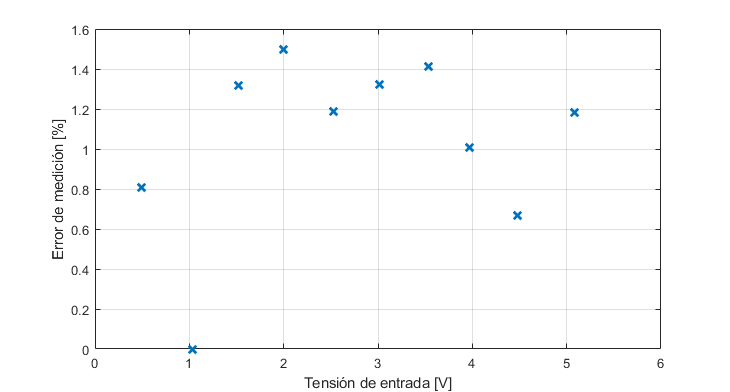
\includegraphics[width=0.9\textwidth]{./Figures/testMonTens.png}
\caption{Error porcentual de la medición de tensión.}
\label{fig:testMonTens}
\end{figure}

Del gráfico se observa que en este rango se tiene un error de medición máximo del 1,5 \% y un valor promedio aproximado del 1,04 \% respecto del valor real.

\subsection{Prueba del monitor de corriente}

Para esta prueba se procede de igual forma que en la subsección \ref{sec:monCorr} pero en lugar de medir la tensión de salida del monitor se toma directamente la lectura de medición de corriente de la pantalla LCD.

Con los datos obtenidos se calcula para cada medición el error porcentual con respecto al valor real de corriente de carga. En la figura \ref{fig:testMonCorr2} se pueden ver los valores computados para distintos valores de corriente en la carga.

\begin{figure}[H]
\centering
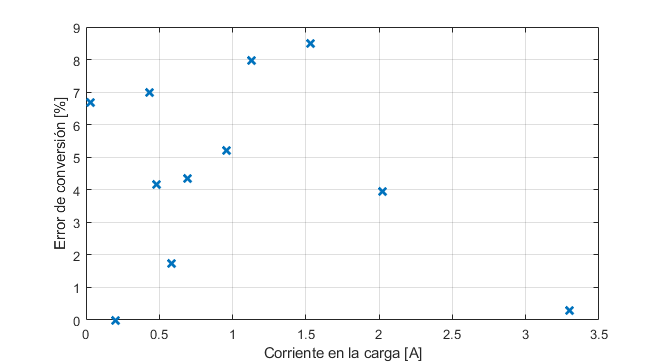
\includegraphics[width=0.9\textwidth]{./Figures/testMonCorr2.png}
\caption{Error porcentual de la medición de corriente.}
\label{fig:testMonCorr2}
\end{figure}

Observando el gráfico se desprende que en este rango se tiene un error de medición máximo del 8,5 \% y un valor promedio aproximado del 4,52 \% respecto del valor real. Estos valores resultan ligeramente mayores a los obtenidos en la sección \ref{sec:monCorr}, lo cual es de esperarse ya que durante el procesamiento digital de los datos se introduce más incerteza (debido a la resolución del ADC) y error de cálculo.

\subsection{Prueba de la pantalla LCD}

En este caso se muestra directamente el LCD durante el funcionamiento normal del programa, lo que implica no solo que la biblioteca desarrollada para la pantalla funciona, si no que los drivers del SPI sobre los que esta implementada también.

En la figura \ref{fig:testLCD} se puede ver la pantalla LCD durante el inicio del programa luego de encender la placa. Como se puede ver, contiene texto y rectángulos de distintos colores, lo que implica el uso de la mayoría de las funciones implementadas en la biblioteca.

\begin{figure}[H]
\centering
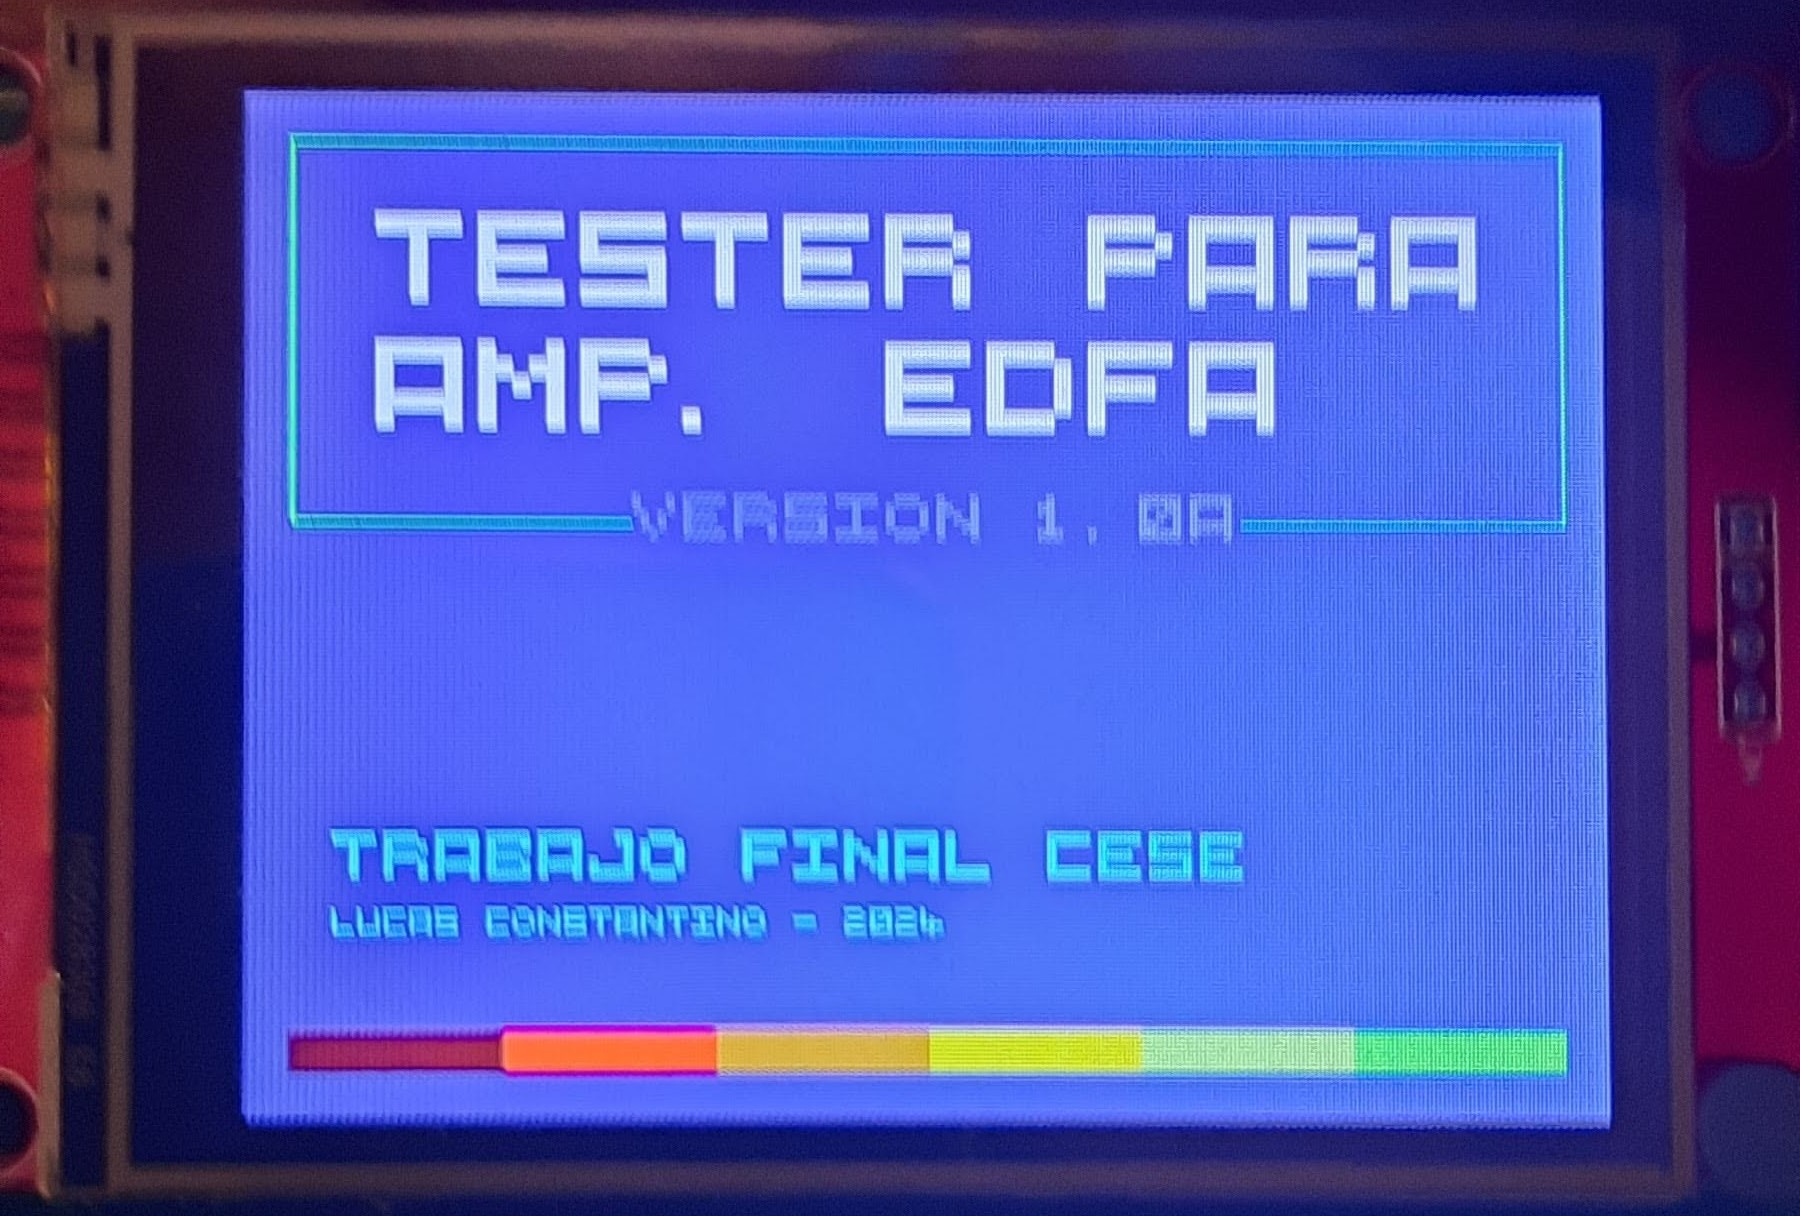
\includegraphics[width=0.8\textwidth]{./Figures/testLCD.jpg}
\caption{Pantalla LCD durante el encendido de la placa.}
\label{fig:testLCD}
\end{figure}

\subsection{Prueba de la consola de control}

La consola de control se encuentra implementada sobre el driver de la UART por lo que al validar el funcionamiento de esta también se estaría validando el del funcionamiento del driver.

Para ello lo que se hace es, mediante el emulador de puertos PuTTY, enviar mediante UART distintos comandos al microcontrolador y verificar que tienen el efecto deseado en la placa. En la figura \ref{fig:pruebaConsola} se puede ver la terminal luego de la ejecución de varios comandos.

\begin{figure}[H]
\centering
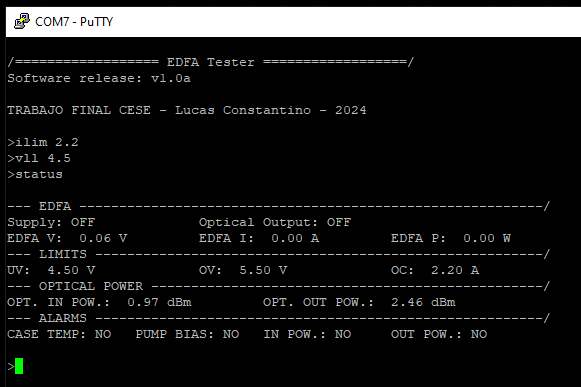
\includegraphics[width=0.9\textwidth]{./Figures/pruebaConsola.png}
\caption{Uso de la consola de control.}
\label{fig:pruebaConsola}
\end{figure}

\section{Pruebas de integración}
\label{sec:pruebasInt}

Las pruebas de integración tienen como objetivo verificar el cumplimiento de los requerimientos establecidos en el documento \citep{DOC_REQ} y mencionados en la sección \ref{sec:reqs}. Al hacer esto se valida la correcta interacción entre el hardware y el firmware, es decir, el funcionamiento del sistema como una unidad.

\subsection{Funcionamiento normal}

En la figura \ref{fig:funcNorm} se puede ver el estado de la pantalla LCD durante el funcionamiento normal, con el amplificador alimentado, su salida óptica prendida y ninguna alarma activa.

\begin{figure}[H]
\centering
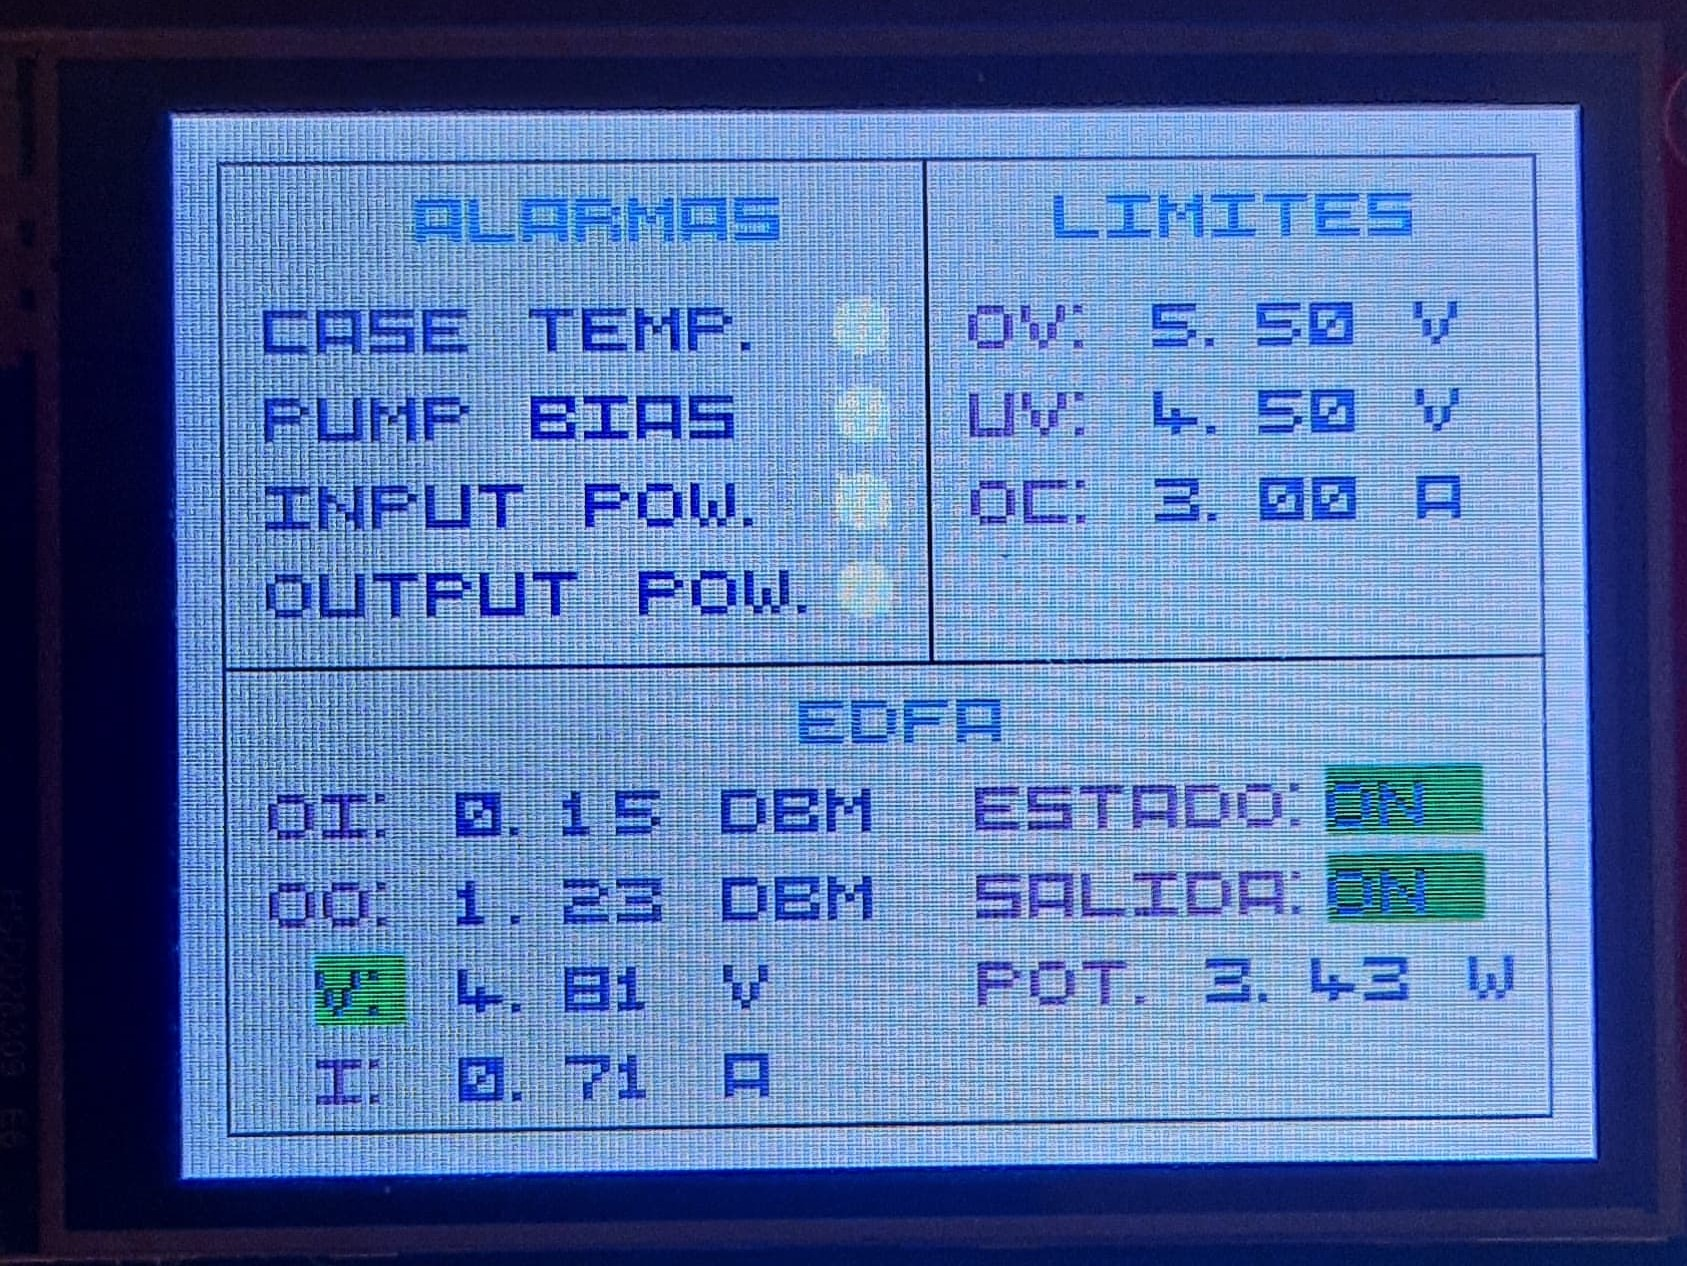
\includegraphics[width=0.75\textwidth]{./Figures/funcNorm.jpg}
\caption{Pantalla LCD durante funcionamiento normal.}
\label{fig:funcNorm}
\end{figure}

De aquí se observa que los valores límites, las alarmas y las variables medidas se actualizan con la frecuencia pretendida en el programa.

\subsection{Detección de alarmas}

Cuando alguna de las alarmas se activa mientras la salida óptica del amplificador permanece encendida, esta se debe apagar inmediatamente mediante la señal de control OUT\_POW\_MUTE, ya que de no hacerlo, esto podría dañar el EDFA.

En la figura \ref{fig:detecAlarm2} se puede ver la conmutación de la señal de control OUT\_POW\_MUTE (canal D1 en rojo) cuando la señal de alarma CASE\_TEMP\_ALARM se activa (canal D0 en blanco). Ambas señales son activas en nivel alto.

\begin{figure}[H]
\centering
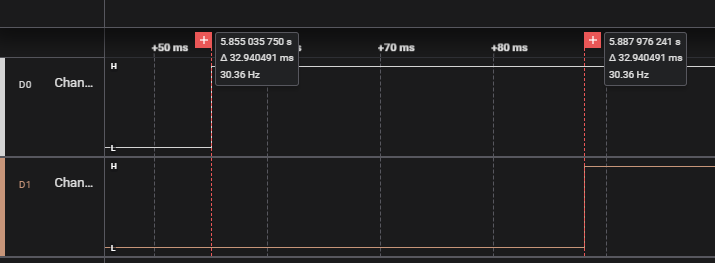
\includegraphics[width=1\textwidth]{./Figures/detecAlarm2.png}
\caption{Detección de alarma y apagado de salida óptica.}
\label{fig:detecAlarm2}
\end{figure}

En la figura anterior se puede observar que el tiempo de retardo que existe entre la detección de la alarma del EDFA y el apagado de la salida óptica es de aproximadamente 33 ms, valor que cumple con el requerimiento 4.2 especificado en la sección \ref{sec:reqs}.

En la figura \ref{fig:detecAlarm} se puede ver el estado de la pantalla LCD luego de la detección de la alarma. El amplificador permanece alimentado pero su salida apagada.

\begin{figure}[H]
\centering
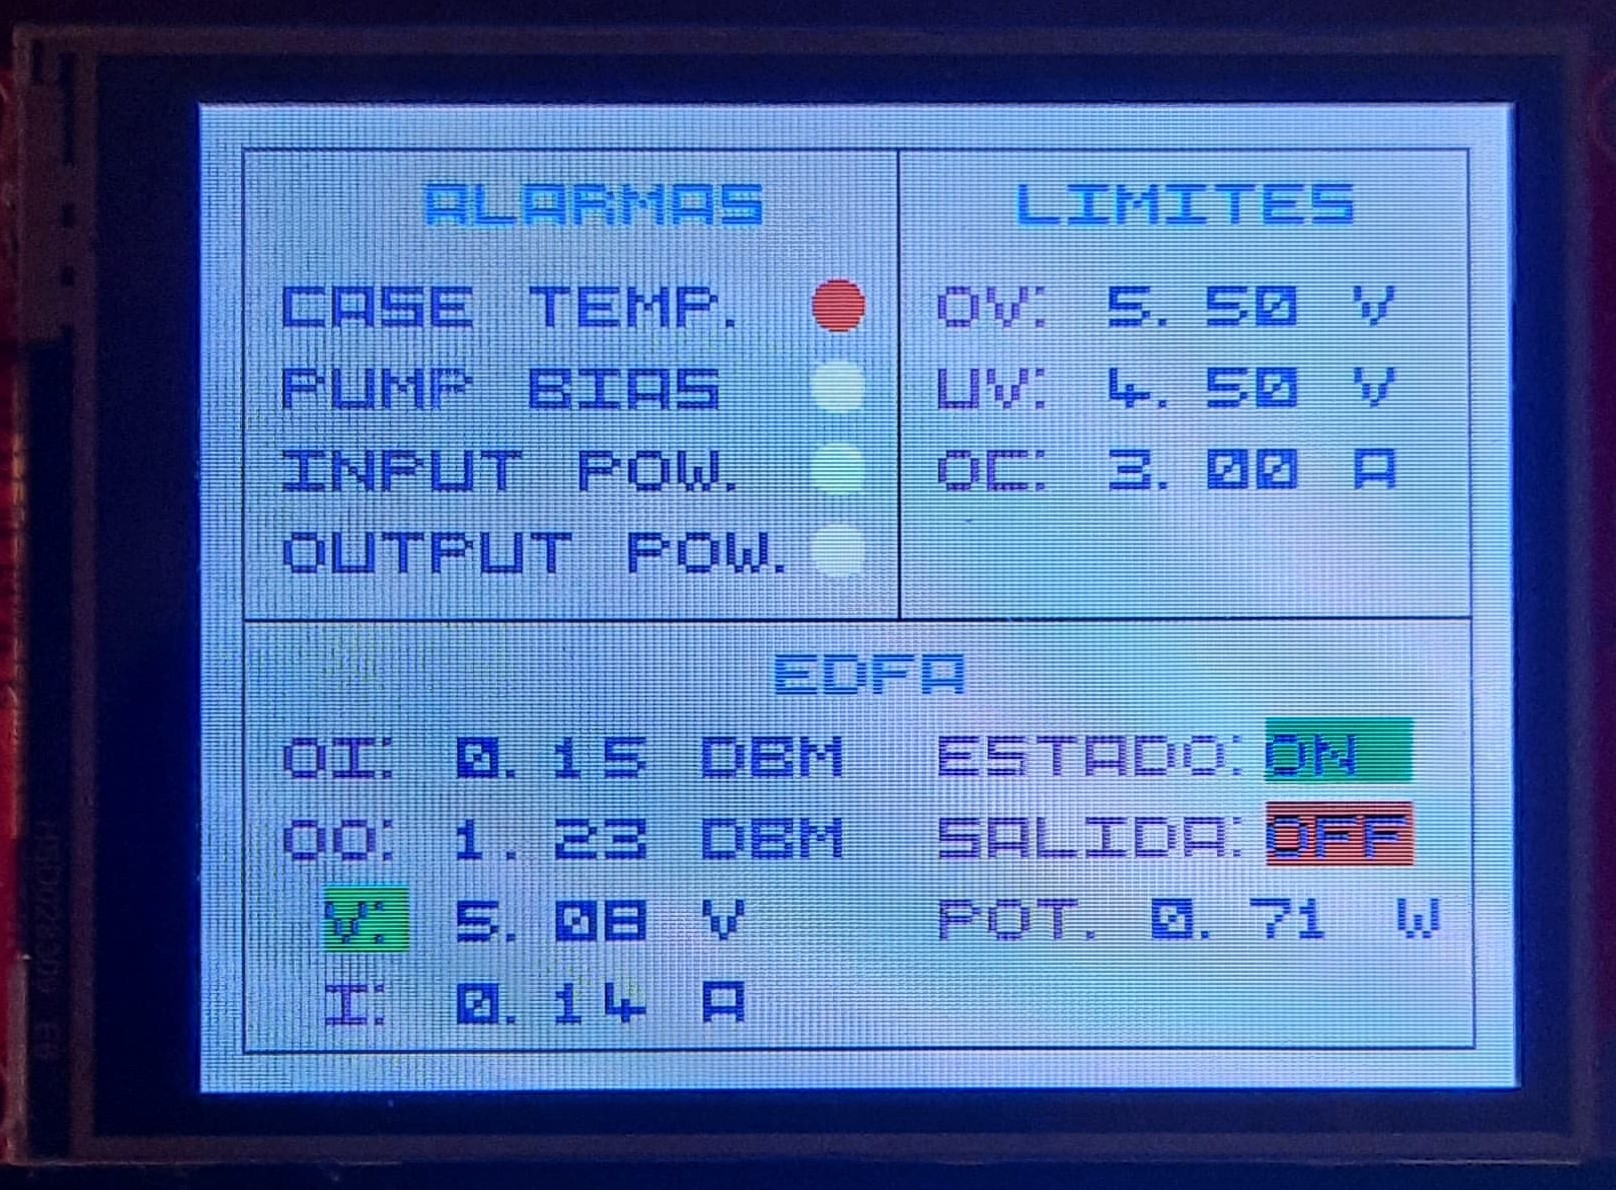
\includegraphics[width=0.75\textwidth]{./Figures/detecAlarm.jpg}
\caption{Pantalla LCD luego de detección de alarma.}
\label{fig:detecAlarm}
\end{figure}

\subsection{Detección de sobrecorriente}

Al igual que para el caso de la detección de alarmas, la detección de una sobrecorriente también debe procesarse rápidamente. En este caso, se asoció la señal de alarma del monitor de corriente a una interrupción en el programa, y se midió el retardo entre el momento en que se activa dicha señal y la desactivación de la señal que controla el relé de alimentación.

En la figura \ref{fig:detecOC} se puede ver la conmutación de la señal que controla la activación del relé (canal D1 en rojo) luego de que la señal de alarma del monitor de corriente se activa (canal D0 en blanco). En este caso la alarma es activa en nivel bajo.

\begin{figure}[H]
\centering
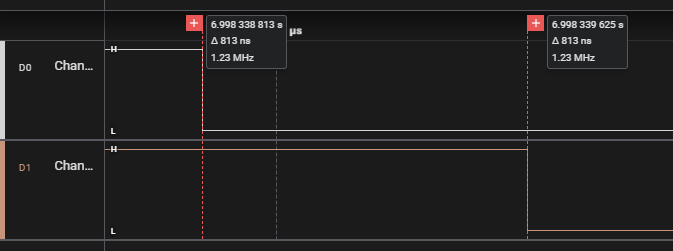
\includegraphics[width=1\textwidth]{./Figures/detecOC.png}
\caption{Detección de sobrecorriente y desconexión del EDFA.}
\label{fig:detecOC}
\end{figure}

Se puede observar que el tiempo de retardo que existe entre la detección de la sobrecorriente y la desconexión del relé es menor a 1~\textmu s, valor que cumple holgadamente con el requerimiento 4.1 especificado en la sección \ref{sec:reqs}.

\section{Comparación del prototipo con el producto existente}

En la tabla \ref{tab:comparacionDisp} se puede ver una comparación entre las funcionalidades del producto existente y las del prototipo desarollado en este trabajo.

\begin{table}[H]
	\centering
	\caption{Comparación entre el dispositivo implementado y el existente.}
	\begin{tabular}{p{6cm} c c}
		\toprule
		\textbf{Característica} & \textbf{Producto existente} & \textbf{Dispositivo desarrollado} \\
		\midrule
		Interfaz UART	& Sí	& Sí \\
		Testigo de alarmas	& Sí	& Sí \\
		Llaves para señales de control		& Sí	& Sí \\
		Alimentación de EDFA				& Sí	& Sí \\
		Detección de sobrecorriente	& No & Sí \\
		Detección de sobretensión		& No & Sí \\
		Detección de baja tensión		& No & Sí \\
		Protección de potencia óptica de entrada	& No & Sí \\
		Protección de potencia óptica de salida		& No & Sí \\
		Desconexión automática de EDFA en caso de alarma & No & Sí \\
		Protección contra descarga electrostática en pines & No & Sí \\
		\bottomrule
		\hline
	\end{tabular}
	\label{tab:comparacionDisp}
\end{table}

\section{Cumplimiento de requerimientos}

